\everymath{\displaystyle}
\documentclass{beamer}
% \documentclass[handout]{beamer}

%\usepackage[pdftex]{color,graphicx}
\usepackage{amsmath,amssymb,amsfonts}

\mode<presentation>
{
  % \usetheme{Darmstadt}
  % \usetheme[hideothersubsections]{Hannover}
  % \usetheme[hideothersubsections]{Goettingen}
  \usetheme[hideothersubsections, right]{Berkeley}

  \usecolortheme{seahorse}
  % \usecolortheme{dolphin}
  \usecolortheme{rose}
  % \usecolortheme{orchid}

  \useinnertheme[shadow]{rounded}

  % \setbeamercovered{transparent}
  \setbeamercovered{invisible}
  % or whatever (possibly just delete it)
}

\mode<handout>{
  \setbeamercolor{background canvas}{bg=black!5}
  \usepackage{pgfpages}
  \pgfpagesuselayout{4 on 1}[a4paper,border shrink=5mm, landscape]
}

\usepackage[brazilian]{babel}
% or whatever

% \usepackage[latin1]{inputenc}
\usepackage[utf8]{inputenc}
% or whatever

\usepackage{times}
%\usepackage[T1]{fontenc}
% Or whatever. Note that the encoding and the font should match. If T1
% does not look nice, try deleting the line with the fontenc.


\title[Encerramento] % (optional, use only with long paper titles)
{Encerramento}

\subtitle
{Até mais, e obrigado pelo peixe} % (optional)

\author%[] % (optional, use only with lots of authors)
{Felipe Figueiredo}% \and S.~Another\inst{2}}
% - Use the \inst{?} command only if the authors have different
%   affiliation.

\institute[] % (optional, but mostly needed)
{
}
  % \inst{1}%
  % Department of Computer Science\\
  % University of Somewhere
  % \and
  % \inst{2}%
  % Department of Theoretical Philosophy\\
  % University of Elsewhere}
% - Use the \inst command only if there are several affiliations.
% - Keep it simple, no one is interested in your street address.

\date%[] % (optional)
{}

% \subject{Talks}
% This is only inserted into the PDF information catalog. Can be left
% out. 



% If you have a file called "university-logo-filename.xxx", where xxx
% is a graphic format that can be processed by latex or pdflatex,
% resp., then you can add a logo as follows:

\pgfdeclareimage[height=1.6cm]{university-logo}{../logo}
\logo{\pgfuseimage{university-logo}}



% Delete this, if you do not want the table of contents to pop up at
% the beginning of each subsection:
\AtBeginSubsection[]
%\AtBeginSection[]
{
  \begin{frame}<beamer>{Sumário}
    \tableofcontents[currentsection,currentsubsection]
  \end{frame}
}


% If you wish to uncover everything in a step-wise fashion, uncomment
% the following command: 

% \beamerdefaultoverlayspecification{<+->}

\usepackage[normalem]{ulem}

\begin{document}

\begin{frame}
  \titlepage
\end{frame}

\begin{frame}{Sumário}
  \tableofcontents
  % You might wish to add the option [pausesections]
\end{frame}


%% Template
% \section{}

% \subsection{}

% \begin{frame}{}
%   \begin{itemize}
%   \item 
%   \end{itemize}
% \end{frame}

% \begin{frame}
%   \begin{columns}
%     \begin{column}{5cm}
%     \end{column}
%     \begin{column}{5cm}
%     \end{column}
%   \end{columns}
% \end{frame}

% \begin{frame}{}
%   \includegraphics[height=0.4\textheight]{file1}
%   \includegraphics[height=0.4\textheight]{file2}
%   \includegraphics[height=0.4\textheight]{file3}
%   \begin{figure}
%     \caption{}
%   \end{figure}
% \end{frame}

% \begin{frame}{}
%   \begin{definition}
%   \end{definition}
%   \begin{example}
%   \end{example}
%   \begin{block}{Exercício}
%   \end{block}
% \end{frame}

\begin{frame}{\scriptsize Discussão da aula passada}
  \begin{block}{}
    Discussão da leitura obrigatória da aula passada
  \end{block}
  \begin{center}
    \vfill
    \invisible{
\includegraphics[height=.5\textheight]{Encerramento/arya-nottoday}}
  \end{center}
\end{frame}

\begin{frame}{\scriptsize \sout{Discussão da aula passada}}
  \begin{block}{}
    \sout{Discussão da leitura obrigatória da aula passada}
  \end{block}
  \begin{center}
    \vfill
    
\includegraphics[height=.5\textheight]{Encerramento/arya-nottoday}
  \end{center}
\end{frame}

\section{Agradecimentos}

\begin{frame}{\scriptsize }
  \begin{center}
    Hoje é dia de {\bf eu} agradecer ao empenho de todos vocês
  \end{center}
\end{frame}

\section{Recapitulação}

\begin{frame}{\scriptsize A temporada até aqui}
  \begin{center}
    
\includegraphics[width=\textwidth]{Encerramento/theroadsofar}
  \end{center}
\end{frame}

\begin{frame}{\scriptsize Muito conteúdo}
  \begin{enumerate}
    \tiny
  \item Introdução

    % {\tiny Análise de Dados}
    \bigskip
  \item Intervalos de Confiança de proporções

    % {\tiny Incertezas de dados categóricos}
  \item Variabilidade

    % {\tiny Incertezas de dados numéricos}
  \item A distribuição Normal

    % {\tiny Distribuição Normal, e IC da média}
    \bigskip
  \item Comparando médias de 2 grupos

    % {\tiny Intervalos de Confiança da diferença entre as médias}
  \item Comparando ICs de proporções

    % {\tiny A Razão de Chances e o Risco Relativo}
  \item Significância e Poder

    % {\tiny Testes de Hipóteses, cálculo amostral e p-valor}
  \item Comparação de dois grupos (quantitativo)

    % {\tiny Testes paramétricos para médias}
  \item Comparação de dois grupos (qualitativo)

    % {\tiny Testes para proporções}
    \bigskip
  \item Correlação Linear

    % {\tiny Associação de duas amostras (quantitativa)}
  \item Regressão Linear Simples

    % {\tiny Modelos com desfecho contínuo}
  \item Tópicos em Regressão Logística

    % {\tiny Modelos com desfecho categórico binário}
  \item Comparações múltiplas e ANOVA

    % {\tiny Teste paramétrico para vários grupos (desfecho quantitativo)}
    \bigskip
  \item Métodos não paramétricos

    % {\tiny Ou: o que fazer caso seus dados não sejam normais?}
  \end{enumerate}
\end{frame}

\begin{frame}{\scriptsize Muito conteúdo}
  \begin{enumerate}
    \tiny
  \item Introdução
  \end{enumerate}

  % {\tiny Análise de Dados}
  % \bigskip
  \begin{block}{\scriptsize Módulo 1 -- descrição e inferência de uma variável}
    \begin{enumerate}
      \setcounter{enumi}{1}
      \tiny
    \item Intervalos de Confiança de proporções

      % {\tiny Incertezas de dados categóricos}
    \item Variabilidade

      % {\tiny Incertezas de dados numéricos}
    \item A distribuição Normal

      % {\tiny Distribuição Normal, e IC da média}
    \end{enumerate}
  \end{block}
  \begin{block}{\scriptsize Módulo 2 -- comparação entre duas variáveis}
    \begin{enumerate}
      \setcounter{enumi}{4}
      \tiny
    \item Comparando médias de 2 grupos

      % {\tiny Intervalos de Confiança da diferença entre as médias}
    \item Comparando ICs de proporções

      % {\tiny A Razão de Chances e o Risco Relativo}
    \item Significância e Poder

      % {\tiny Testes de Hipóteses, cálculo amostral e p-valor}
    \item Comparação de dois grupos (quantitativo)

      % {\tiny Testes paramétricos para médias}
    \item Comparação de dois grupos (qualitativo)

      % {\tiny Testes para proporções}
    \end{enumerate}
  \end{block}
  \begin{block}{\scriptsize Módulo 3 -- introdução à modelagem estatística}
    \begin{enumerate}
      \setcounter{enumi}{8}
      \tiny
    \item Correlação Linear

      % {\tiny Associação de duas amostras (quantitativa)}
    \item Regressão Linear Simples

      % {\tiny Modelos com desfecho contínuo}
    \item Tópicos em Regressão Logística

      % {\tiny Modelos com desfecho categórico binário}
    \item Comparações múltiplas e ANOVA

      % {\tiny Teste paramétrico para vários grupos (desfecho quantitativo)}
    \end{enumerate}
  \end{block}
  \begin{enumerate}
    \setcounter{enumi}{13}
    \tiny
  \item Métodos não paramétricos

    % {\tiny Ou: o que fazer caso seus dados não sejam normais?}
  \end{enumerate}
\end{frame}

\begin{frame}{\scriptsize }
  \begin{center}
    Exaustivo

    \vfill
    \visible<2>{\bf né?}
  \end{center}
\end{frame}

\begin{frame}{\scriptsize {\bf Sempre} na última hora}
  \begin{center}
    
\includegraphics[height=.75\textheight]{Encerramento/phdcomics-motivation}

    \vfill
    \visible<2>{\bf né?}
  \end{center}
\end{frame}

\begin{frame}{\scriptsize E o pânico de testes e provas}
  \begin{center}
    
\includegraphics[width=.8\textwidth]{Encerramento/phdcomics-correcao}

    \vfill
    \visible<2>{\bf né?}
  \end{center}
\end{frame}

\begin{frame}
  \begin{center}
    Valeu a pena?

    \vfill
    \visible<2>{\bf *\#*\#*\#*\#**@\#*\#*@*\#*...}
  \end{center}
\end{frame}

\section{Retorno}

\begin{frame}{\scriptsize Módulo 1 -- aulas}
  \begin{enumerate}
    \setcounter{enumi}{1}
  \item Intervalos de Confiança de proporções

    {\tiny Incertezas de dados categóricos}
    \bigskip
  \item Variabilidade

    {\tiny Incertezas de dados numéricos}
    \bigskip
  \item A distribuição Normal

    {\tiny Distribuição Normal, e IC da média}
  \end{enumerate}
\end{frame}

\begin{frame}{\scriptsize Aula 2 -- Intervalos de Confiança de proporções}
  \begin{itemize}
    \footnotesize
  \item Amostra x população

    {\tiny a amostra é representativa da população?}
    \bigskip
  \item Distribuição binomial

    {\tiny histograma da distribuição binomial}
    \bigskip
  \item Análise descritiva de uma variável categórica

    {\tiny Frequências e Proporções}
    \bigskip
  \item Análise inferencial de uma variável categórica

    {\tiny Intervalo de confiança de uma proporção}
  \end{itemize}
\end{frame}

\begin{frame}{\scriptsize Aula 3 -- Variabilidade}
  \begin{itemize}
    \footnotesize
  \item Fontes de variabilidade

    {\tiny é razoável pressupor que a variável tem distribuição Normal?}
    \bigskip
  \item Visualizando o centro e a variabilidade

    {\tiny histograma/boxplot de uma distribuição de dados quantitativos}
    \bigskip
  \item Construção da ideia de dispersão em relação à média

    {\tiny Desvio $\rightarrow$ variância $\rightarrow$ desvio-padrão (DP)}
    \bigskip
  \item Variabilidade

    {\tiny Variância/desvio-padrão e quartis/percentis}
    \bigskip
  \item Análise descritiva de uma variável quantitativa

    {\tiny centro (dispersão) $\rightarrow$ média (DP) ou mediana (IIQ)}
  \end{itemize}
\end{frame}

\begin{frame}{\scriptsize Aula 4 -- A distribuição Normal}
  \begin{itemize}
    \footnotesize
  \item A distribuição Normal

    {\tiny reconhecer as principais características em um histograma}
    \bigskip
  \item A regra empírica

    {\tiny que proporção da população observamos da 1DP da média? 2DP? 3DP?}
    \bigskip
  \item (N grande) distribuição binomial $\rightarrow$ distribuição normal

    {\tiny Vídeo!}
    \bigskip
  \item Análise inferencial de uma variável quantitativa

    {\tiny Erro padrão e Intervalo de confiança de uma média}
  \end{itemize}
\end{frame}

\begin{frame}{\scriptsize Módulo 2 -- aulas}
  \begin{enumerate}
    \setcounter{enumi}{4}
  \item Comparando médias de 2 grupos

    {\tiny Intervalos de Confiança da diferença entre as médias}
    \bigskip
  \item Comparando ICs de proporções

    {\tiny A Razão de Chances e o Risco Relativo}
    \bigskip
  \item Significância e Poder

    {\tiny Testes de Hipóteses, cálculo amostral e p-valor}
    \bigskip
  \item Comparação de dois grupos (quantitativo)

    {\tiny Testes paramétricos para médias}
    \bigskip
  \item Comparação de dois grupos (qualitativo)

    {\tiny Testes para proporções}

  \end{enumerate}
\end{frame}

\begin{frame}{\scriptsize Aula 5 -- Comparando médias de 2 grupos}
  \begin{itemize}
    \footnotesize
  \item Família da distribuições normais + o agregado

    {\tiny Distribuição Normal Padrão (Z) e distribuição t de Student}
    \bigskip
  \item Distribuição t de Student

    {\tiny amostras pequenas, graus de liberdade}
    \bigskip
  \item Comparação das médias de dois grupos independentes

    {\tiny usando análise inferencial -- IC da diferença}
    \bigskip
  \item Comparação das médias de dois grupos pareados

    {\tiny usando análise inferencial -- IC da diferença}
  \end{itemize}
\end{frame}

\begin{frame}{\scriptsize Aula 6 -- Comparando ICs de proporções}
  \begin{itemize}
    \footnotesize
  \item Tipos de estudos (simplificado)

    {\tiny retrospectivo, prospectivo, transversal e experimental}
    \bigskip
  \item Tabulação de duas variáveis binárias

    {\tiny tabelas de contingência}
    \bigskip
  \item Comparação das proporções de dois grupos -- OR

    {\tiny usando análise inferencial -- IC da OR}
    \bigskip
  \item Comparação das proporções de dois grupos -- RR

    {\tiny usando análise inferencial -- IC da RR}
  \end{itemize}
\end{frame}

\begin{frame}{\scriptsize Aula 7 -- Significância e Poder}
  \begin{itemize}
    \footnotesize
  \item Hipóteses científicas x hipóteses estatísticas

    {\tiny a dificuldade em reduzir a pergunta científica em componentes testáveis}
    \bigskip
  \item Poder estatístico

    {\tiny influência do tamanho do efeito, do tamanho do estudo (N) e da variabilidade}
    \bigskip
  \item teste de hipóteses

    {\tiny hipótese nula, hipótese alternativa e a dificuldade da ``lógica invertida''}
    \bigskip
  \item Erros tipo I e tipo II

    {\tiny Falso positivo ($\alpha$) e falso negativo ($\beta$)}
    \bigskip
  \item O p-valor

    {\tiny a dificuldade em abstrair ``infinitos experimentos idênticos''}
  \end{itemize}
\end{frame}

\begin{frame}{\scriptsize Aula 8 -- Comparação de dois grupos (quantitativo)}
  \begin{itemize}
    \footnotesize
  \item Comparação das médias de dois grupos independentes

    {\tiny usando o teste t para duas amostras}
    \bigskip
  \item Comparação das médias de dois grupos pareados

    {\tiny usando o teste t para uma amostra}
    \bigskip
  \item Dinâmica em aula -- processo construtivo

    {\tiny primeiro desafio em selecionar um entre dois métodos}
    \bigskip
  \end{itemize}
\end{frame}

\begin{frame}{\scriptsize Aula 9 -- Comparação de dois grupos (qualitativo)}
  \begin{itemize}
    \footnotesize
  \item Expectativa x Realidade -- teste qui-quadrado para uma amostra

    {\tiny quanta discrepância observamos em relação ao esperado?}
    \bigskip
  \item Comparação das proporções de dois grupos

    {\tiny usando o teste qui-quadrado para duas amostras}
    \bigskip
  \item Comparação das proporções de dois grupos

    {\tiny usando o teste exato de Fisher para duas amostras}
    \bigskip
  \item Visualização de tabelas de contingência

    {\tiny gráfico de barras de duas amostras, e porque não usar gráfico de pizza}
    \bigskip
  \item Tabelas de contingência maiores

    {\tiny estes testes funcionam para qualquer número de categorias}
  \end{itemize}
\end{frame}

\begin{frame}{\scriptsize Módulo 3 -- aulas}
  \begin{enumerate}
    \setcounter{enumi}{9}
  \item Correlação Linear

    {\tiny Associação de duas amostras (quantitativa)}
    \bigskip
  \item Regressão Linear Simples

    {\tiny Modelos com desfecho contínuo}
    \bigskip
  \item Tópicos em Regressão Logística

    {\tiny Modelos com desfecho categórico binário}
    \bigskip
  \item Comparações múltiplas e ANOVA

    {\tiny Teste paramétrico para vários grupos (desfecho quantitativo)}
  \end{enumerate}
\end{frame}

\begin{frame}{\scriptsize Aula 10 -- Correlação Linear}
  \begin{itemize}
    \footnotesize
  \item Correlação não implica causalidade

    {\tiny quatro perguntas norteadoras para interpretação}
    \bigskip
  \item Reconhecer tendências lineares, não lineares ou ausência

    {\tiny usando o gráfico de dispersão}
    \bigskip
  \item Coeficiente de correlação linear de Pearson

    {\tiny direção e magnitude da associação linear}
    \bigskip
  \item Tópicos em causalidade

    {\tiny \em spurious correlations!}
    \bigskip
  \item Correlação não implica causalidade

    {\tiny nunca é demais repetir}
  \end{itemize}
\end{frame}

\begin{frame}{\scriptsize Aula 11 -- Regressão Linear Simples}
  \begin{itemize}
    \footnotesize
  \item Relação linear explícita entre duas variáveis contínuas

    {\tiny reta de melhor ajuste -- simplifica a interpretação do problema}
    \bigskip
  \item Diagnóstico do modelo proposto

    {\tiny análise de resíduos}
    \bigskip
  \item Quanta variância é explicada pelo modelo proposto?

    {\tiny coeficiente de determinação (R2)}
    \bigskip
  \item Predizendo valores não observados

    {\tiny estimativa pontual e IC usando o modelo proposto}
    \bigskip
  \item Heterogeneidade da variância ao longo da escala observada

    {\tiny casos patológicos -- inviabilidade do modelo}
  \end{itemize}
\end{frame}

\begin{frame}{\scriptsize Aula 12 -- Tópicos em Regressão Logística}
  \begin{itemize}
    \footnotesize
  \item Tópicos em regressão linear múltipla

    {\tiny ajustando estimativa da RLS com cofatores sabidamente relevantes}
    \bigskip
  \item Visualizações de dados mais complexas

    {\tiny codificar cofatores em cores para identificar padrões}
    \bigskip
  \item Tópicos em regressão logística (múltipla)

    {\tiny estimativa da OR ajustada por cofatores sabidamente relevantes}
    \bigskip
  \item (bônus) como tabular dados quantitativos e qualitativos

    {\tiny tabela de dados no Excel!}
  \end{itemize}
\end{frame}

\begin{frame}{\scriptsize Aula 13 -- Comparações múltiplas e ANOVA}
  \begin{itemize}
    \footnotesize
  \item O problema dos múltiplos testes

    {\tiny o nível de significância é artificialmente inflacionado}
    \bigskip
  \item Comparação das médias de três (ou mais) grupos independentes

    {\tiny usando a Análise de Variâncias com um fator}
    \bigskip
  \item Comparação das variâncias de dois grupos independentes

    {\tiny usando o teste F}
    \bigskip
  \item Ajuste de p-valor no pós-teste

    {\tiny os métodos de Bonferroni e Tukey}
    \bigskip
  \item Análise de Variâncias com dois fatores

    {\tiny comparação de três ou mais médias ajustando por um cofator relevante}
  \end{itemize}
\end{frame}

\section{A disciplina foi desafiadora}

\begin{frame}{O fim está próximo}
  \begin{center}
    
\includegraphics[height=.75\textheight]{Encerramento/dogdaysareover}

    \vfill
    \visible<2>{\bf ufa...}
  \end{center}
\end{frame}

\begin{frame}{E você foi forte}
  \begin{center}
    
\includegraphics[height=.75\textheight]{Encerramento/naodesista3}

    \vfill
    \visible<2>{\bf tá?}
  \end{center}
\end{frame}

\section{Perspectivas do futuro}

\begin{frame}{\scriptsize }
  \begin{center}
    Você recebeu muita informação...

    \bigskip
    \bigskip
    \footnotesize
    ... mas com isso ganhou muito vocabulário
  \end{center}
\end{frame}

\begin{frame}[label=exemplo-varios]{\scriptsize Na prática...}
  \begin{center}
    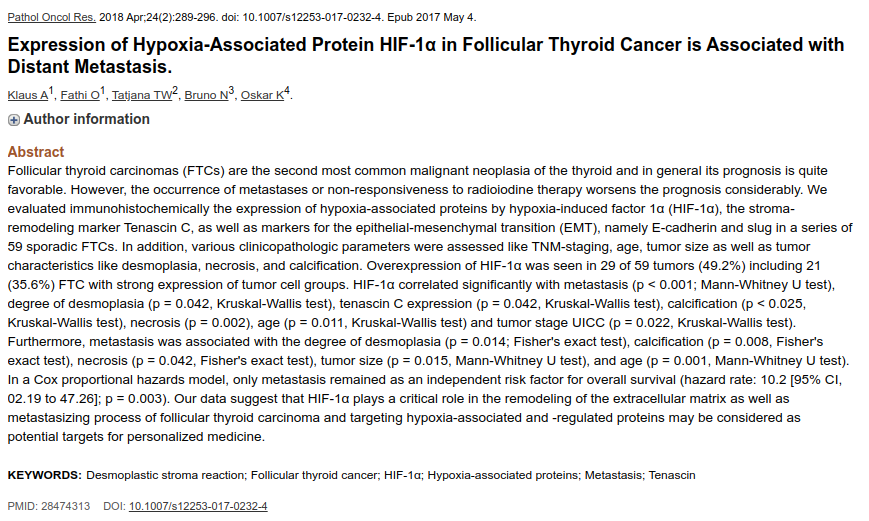
\includegraphics[width=\textwidth]{Cap37-38/exemplo-varios}
  \end{center}
\end{frame}

\begin{frame}{\scriptsize }
  \begin{center}
    Essa experiência te transformou...?

    \bigskip
    \bigskip
    \footnotesize
    \visible<2>{Sente-se mais apto(a) para {\bf ler criticamente} sua literatura?}
  \end{center}
\end{frame}

\begin{frame}{\scriptsize }
  \begin{center}
    Espero que sim!

    \bigskip
    {\footnotesize Meu esforço foi para selecionar os métodos mais comuns...}

    \vfill
    \visible<2>{\tiny ... e ocultar pelo menos algumas das armadilhas mais abstratas}
  \end{center}
\end{frame}

\begin{frame}{\scriptsize }
  \begin{center}
    Obrigado por tudo! Até mais...

    % \bigskip
    \bigskip
    ... e obrigado pelo peixe!
    \bigskip
    \bigskip

    
\includegraphics[height=0.4\textheight]{Encerramento/thanksfish}
    \vfill
    % \hfill \tiny (nenhum golfinho foi ferido na produção desta aula)
  \end{center}
\end{frame}

\end{document}
